\documentclass[11pt]{article}
% Time-stamp: <homework-02.tex, saved on Fri, Sep 14, 2007 at 12:46pm>
\usepackage[margin=1in, head=1in]{geometry}
\usepackage{amsmath, amssymb, amsthm}
\usepackage{fancyhdr}
\usepackage{graphicx}
\usepackage{pgfplots}

%\usepackage{pdfsync}
\addtolength{\textwidth}{.5in}
\addtolength{\leftmargin}{-1in}
\addtolength{\textheight}{.5in}
\addtolength{\topmargin}{-0.5in}

%\pagestyle{fancy}
%\lhead{MATH 200X }
%\chead{Fall 2007}
%\rhead{FINAL EXAM}
%\lfoot{}
%\cfoot{\thepage}
%\rfoot{}

\setcounter{secnumdepth}{0}
%\renewcommand{\theenumi}{\alph{enumi}}
%\renewcommand{\emptyset}{\varnothing}
\newcommand{\R}{\mathbb{R}}
\newcommand{\N}{\mathbb{N}}
\newcommand{\Z}{\mathbb{Z}}
\newcommand{\clm}{\par\textit{Claim:}\par}
\newcommand{\diam}{\mathrm{diam}}
\newcommand{\sect}{\textsection}

\parindent=0in
\parskip=0.5\baselineskip

\begin{document} 

\begin{center}MATH 156: Precalculus  \\ Fall 2015 \\ Worksheet \sect 1.11: Solving Equations and Inequalities Graphically\end{center}

\hrulefill

By the end of this section you must know how to:
\begin{itemize}
\item solve inequalities graphically
\item solve equations graphically
\end{itemize}

\hrulefill

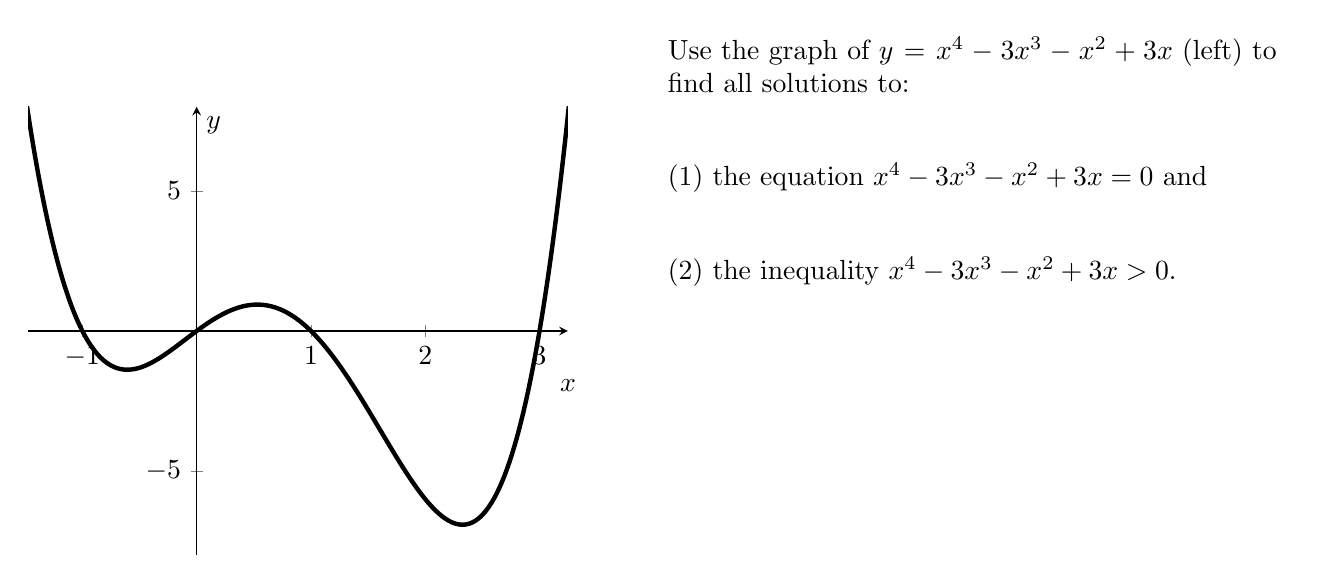
\begin{tikzpicture}[scale=1]
\begin{axis}[
        axis x line=middle, 
        axis y line=middle, 
        ymax=8, 
        ymin=-8,
        ylabel=$y$, 
        x label style={at={(current axis.right of origin)},anchor=north, below=5mm},
         xlabel=$x$,
        %x label style={at={(axis description cs:4,-1)},anchor=north},
        ]
    \addplot[domain=-2:4, samples=400, black, ultra thick]  {x^4 - 3*x^3-x^2+3*x};
\end{axis}
\node[text width=8cm, anchor=west, right] at (8,5)
    {Use the graph of $y=x^4-3x^3-x^2+3x$ (left) to find all solutions to: \\
    \vspace{.3in}
    (1) the equation $x^4-3x^3-x^2+3x=0$ and \\
    \vspace{.3in}
    (2) the inequality $x^4-3x^3-x^2+3x>0.$ };
\end{tikzpicture}

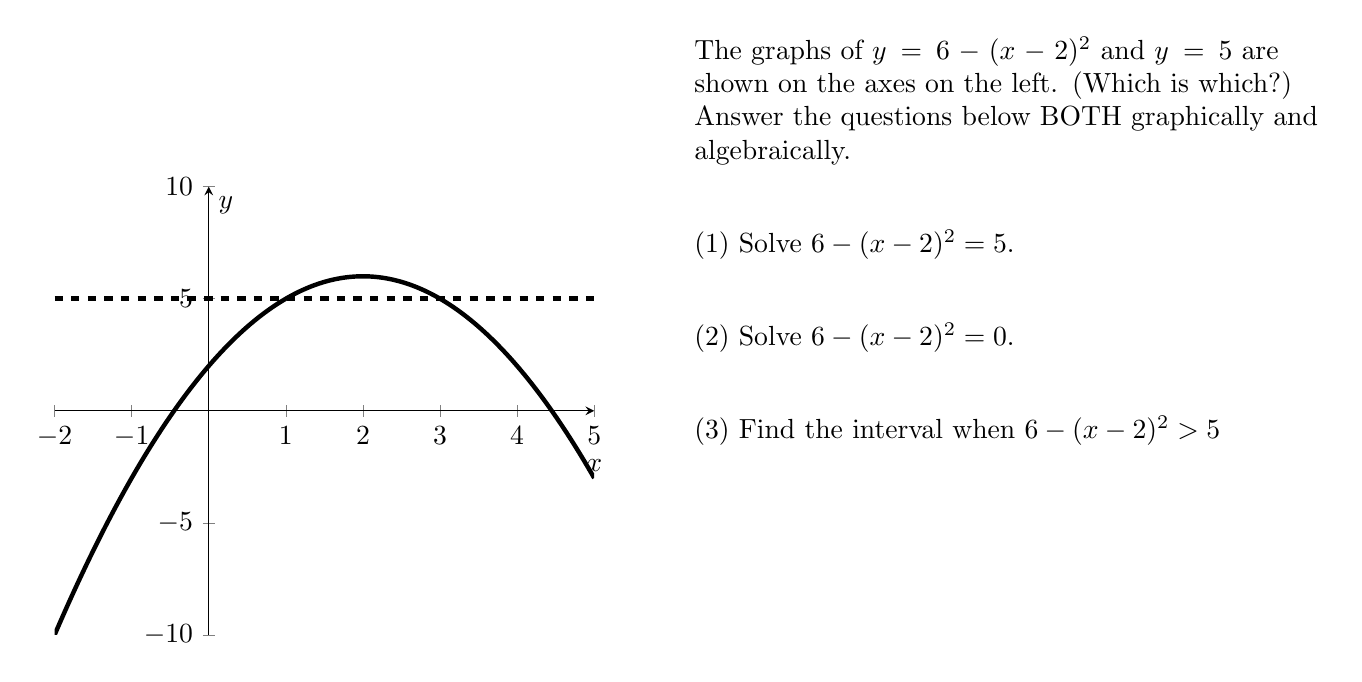
\begin{tikzpicture}[scale=1]
\begin{axis}[
        axis x line=middle, 
        axis y line=middle, 
        ymax=10, 
        %ymin=-8,
        xmax=5,
        xmin=-2,
        ylabel=$y$, 
        x label style={at={(current axis.right of origin)},anchor=north, below=5mm},
         xlabel=$x$,
        %x label style={at={(axis description cs:4,-1)},anchor=north},
        ]
    \addplot[domain=-2:5, samples=400, black, ultra thick]  {6-(x-2)^2};
    \addplot[domain=-2:5, black, ultra thick, dashed]  {5};
\end{axis}
\node[text width=8cm, anchor=west, right] at (8,5)
    {The graphs of $y=6-(x-2)^2$ and $y=5$ are shown on the axes on the left.  (Which is which?) Answer the questions below BOTH graphically and algebraically. \\
    \vspace{.3in}
    (1) Solve $6-(x-2)^2=5.$\\
    \vspace{.3in}
    (2) Solve $6-(x-2)^2=0.$ \\
    \vspace{.3in}
    (3) Find the interval when $6-(x-2)^2>5$\\
    };
\end{tikzpicture}

Problem: On the same set of axes, graph $y=x^2$ and $y=1-x.$ Use the graphs to answer the questions below.
\begin{enumerate}
\item Solve $x^2=1-x.$
\item Describe the interval of the real line such that $1-x \geq x^2.$
\end{enumerate}

\end{document}
